% document type
\documentclass[12pt]{article}

% packages
\usepackage[total={170mm,230mm}]{geometry}
\usepackage[utf8]{inputenc}
\usepackage[T1]{fontenc}
\usepackage[russian]{babel}
\usepackage{graphicx}
\usepackage{amssymb}
\usepackage{amsfonts}
\usepackage{amsmath}
\usepackage{amsthm}
\usepackage{physics}
\usepackage{nicefrac}
\usepackage{cancel}
\usepackage{hyperref}
\usepackage{cmap}

\newcommand*{\figref}[2][]{\hyperref[#2]{Рис.~\ref*{#2}#1}}
% \newcommand*{\tblref}[1]{\hyperref[#1]{Table~\ref*{#1}}}
\newcommand*{\secref}[1]{\hyperref[#1]{Section~\ref*{#1}}}
% \newcommand*{\secsref}[1]{\hyperref[#1]{Sections~\ref*{#1}}}
% \newcommand*{\introref}[1]{\hyperref[#1]{Introduction}}

\begin{document}
	\begin{titlepage}
    \begin{center}
    % \vspace{-3em}
    {\small\textsc{Нижегородский государственный университет имени Н.\,И. Лобачевского}}
    \vskip 2pt \hrule \vskip 3pt
    {\small\textsc{Высшая школа общей и прикладной физики}}

    \vfill


    {{\large Отчет по лабораторной работе}\vskip 12 pt {\Large \bfseries Низкочастотные процессы в многомодовом твердотельном лазере}}

        
    \vspace{2cm}
    {\large Работу выполнили студенты \\[0.5em]{\Large \bfseries Поляков Андрей, Козлов Александр}}

    \end{center}

    \vfill

    \begin{center}
    {Нижний Новгород, \today}
    \end{center}
\end{titlepage}
	\setcounter{page}{2}

	\tableofcontents
	\newpage

	\section{Схема установки}

	\begin{figure}[tb]
		\centering
		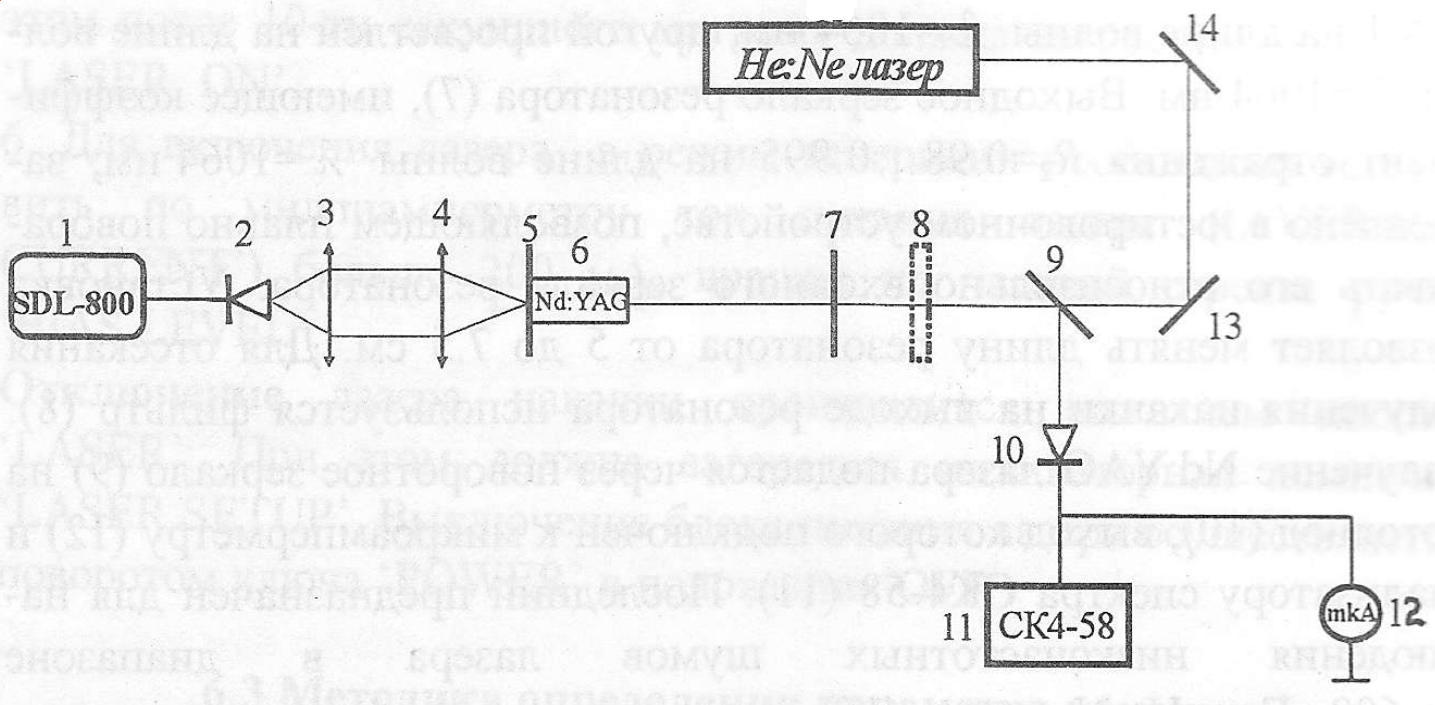
\includegraphics[width=\textwidth]{../figures/scheme.png}
		\caption{Схема установки.}
		\label{fig:scheme}
	\end{figure}

	Схема экспериментальной установки представлена на \figref{fig:scheme}. В качестве источника накачки используется полупроводниковый лазер (2) со следующими характеристиками
	\begin{enumerate}
		\item длина волны генерации $810\.\text{нм}$;
		\item пороговый ток питания $200\.\text{мА}$;
		\item максимальная мощность излучения $0.5\.\text{Вт}$;
		\item поляризация излучения линейная, вектор электрического поля лежит в вертикальной плоскости.
	\end{enumerate}

	

	\section{Основные элементы теории}

	\section{Результаты эксперимента с оценкой погрешности и их сравнение с теорией}

	\section{Протокол измерений}
\end{document}